% Chapter 3: Scope of the project

\chapter{\company\ Heatmap }

\label{chapter03}

%-----------------
%   SECTION 3.1
%-----------------

\section{Definition of the problem} \label{problem}

%In any moment, \company\ uses user sessions or user queries to guess trends.
In any team of \company, the user queries and the providers data is compared in order to guess valuable trends for different \nameref{stakeholders}.
\\\\
Found that gap, a bunch of new ideas appeared. After some talks with product owners of different squads and some senior engineers a promising idea showed up:
\\\\
Comparison of \textbf{user demand} and \textbf{flights offered} by airlines, enabling finding \textit{over-requested} routes or airports. 
\\\\
\squad manages a huge amount of data: All flights planned for the next two years, this are more than 75 million records. The database of all user queries in the website or mobile application is even bigger\footnote{For instance, if there were only one query per visitor the database would have 4 million new records per day}. Not much more information needed to say that this is \textbf{Big Data} problem.
\\\\
With \squad's product owner help, we found some use cases for the professing of those 75 million routes and all user session's queries to get some significant results.
\\\\
Provide a visual tool to find routes and airports with much more demand than offer and be able to observe the evolution of it through time:

\begin{itemize}
  \item A route or airport with a lot of demand but not enough offer to cover it will be \textbf{over-requested}.
  \item A route or airport with much more offer but not that amount of demand will be \textbf{non-profitable}.
\end{itemize}

%-----------------
%   SECTION 3.2
%-----------------

\section{Scope}

Merging both data sources (providers and users) generates a lot of new valuable data with a lot of different application: From simply selling it to stakeholders, to complex deep learning systems.
\\\\
The final goal of this project is displaying the comparison in a simple Web UI for Marketing Squads or Tribes. This can be split in three smaller goals or components:

\subsection{Pipeline}

Distributed application that maps and merge all the data from both sources in its given format, to the required data model.
\\\\
The pipeline reads from \nameref{mp_engine} and \nameref{data_tribe} services. Then, the pipeline, maps the provider and user data to the desired data model. The new entities are stored in a database where the service will read from.
\\\\
The application will be split in two sub applications, one for providers' data and other for users'. So both can vary independently without depending on the each others' sources and changes may have in the future.

\subsection{Service}

Simple HTTP Service with a basic Application Programming Interface to \textbf{get} Pipeline's results. The service will have an internal endpoint only available for other \company\ applications or developers.

\subsection{Visual representation} \label{visual_representation}

Website with a visual representation of the data. There are plenty of ways to draw charts and maps visualizations.
\\\\
The Web UI will be composed by three main pages:

\subsubsection*{World Map}

Interactive world map with all airports represented with a dot. The radius of the dot depends on the amount of flights it operates.
\\\\
The user will be able to select an airport set a date and go to \nameref{chart_visualization} page. Another option is to select two airports, first the origin, then the destination, set a date and go to the \nameref{chart_visualization} page. If the user does not want to select the entity through the map, he/she can search it using the \nameref{browser}

\begin{figure}[H]
\centering
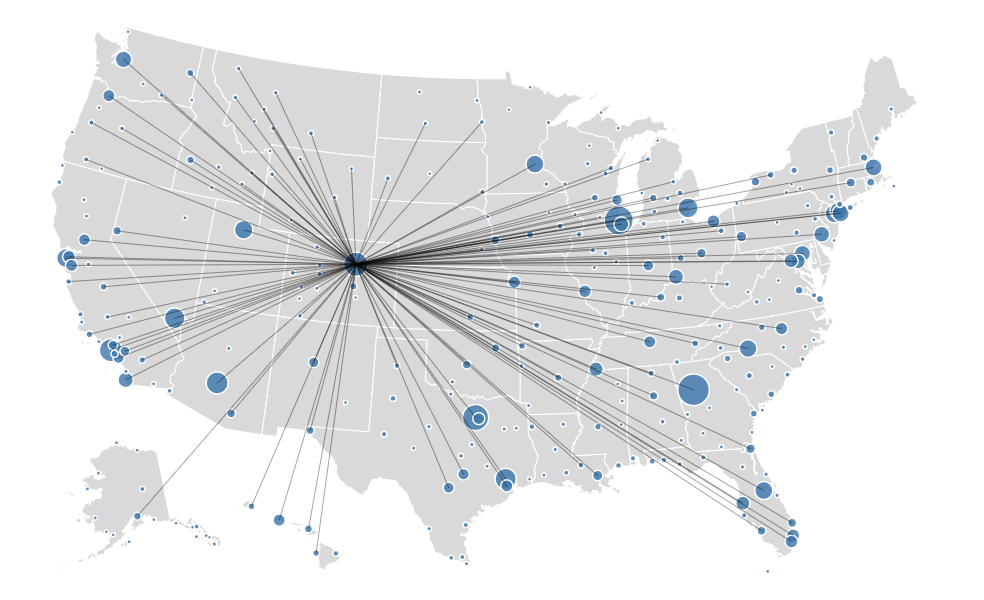
\includegraphics[scale=0.25]{resources/us-map-example01.png}
\caption{Example of how the world map style. Only displaying the US make it look clearer.}
\end{figure}

\subsubsection*{Browser} \label{browser}

Simple browser with two tabs: \textit{Route} and \textit{Airport}. In the route browser will appear three input text fields, one for the origin airport, the second for the destination and the last one for the date. In the airport browser will only appear two input text fields, airport and date.
\\\\
Once the inputs are set, the user will be able to click a \textit{Search} button and move to the next page, \nameref{chart_visualization}.

\subsubsection*{Chart visualization} \label{chart_visualization}

Simple chart with the comparison between providers offer and user demand of the selected entity through time.

\begin{figure}[H]
\centering
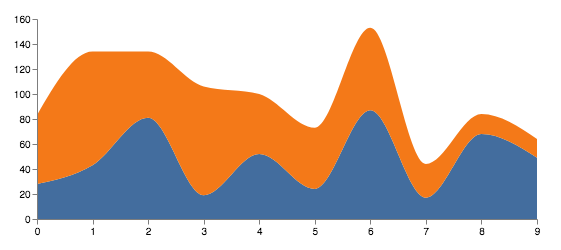
\includegraphics[scale=0.3]{resources/stacked-chart-example01.png}
\caption{Chart mock-up. One color goes for Providers Offer and the other one for User Demand.}
\end{figure}

\subsection{Not list}

It is also important to define what this project will \textbf{not} be.

% WIP
\begin{itemize}
  \item \textbf{Prices} or \textbf{quotes}: In any moment will check for flight prices or quotes.
  \item \textbf{Carriers}, \textbf{cities} and \textbf{countries}: The comparison will be only available between routes and airports, not airlines (carriers), cities nor countries.
  \item \textbf{Create}, \textbf{update} or \textbf{delete} data through the \textbf{Server}: The only input will come from the pipeline. Entities are never deleted or modified in order to keep historical data.
  \item \textbf{Create}, \textbf{update} or \textbf{delete} data through the \textbf{Web UI}: The only input will come from the pipeline. Entities are never deleted or modified in order to keep historical data.
\end{itemize}

%-----------------
%   SECTION 3.3
%-----------------

\section{Risks}

There are several risks can appear while developing the project. Most risks appear because of the dependencies with other tribes and squads, dependencies with other services. In the other hand, all performance risks of the Pipeline can ignored because \company's hardware is enough for big applications like this one.

\subsection{Routes contract}

\squad's routes service is under development and during the Heatmap development the routes' data model may change a little bit. For example, the origin and destination recently changed, in December 2017 their service was giving an \textit{Airport ID}, but now are given in an Airport object with more parameters like IATA Code\cite{iata_code}, Country ID, City ID, etc.

\subsection{Users information}

In the website and mobile application, the user have plenty of different ways to search the perfect flight. The most common one is by origin, destination and date, but he/she can also search by month, by destination. This way the user search flights may be difficult to compare with routes and airports offer because, sometimes, the route is the actual result.
\\\\
The user does not search flights for a given route in a given date. It sets the period of time he/she can travel and \company\ offers cheap destinations.

\subsection{Amount of data}

As explained before in the \nameref{problem}, there is a very big amount of data that need to be mapped\footnote{Simple approximation for one year:
\\
62 thousand routes per week, around 20\% of those routes are new or changed from previous version, this is $62000+12400\times 52 weeks = 706800$ records per year.
\\
In the other hand we have 4 million users every day, supposing the 75\% of them do one simple query (origin, destination and date): $4000000\times365=1460000000$ records.
\\
With a simple data model such as origin (Integer, 4 bytes), destination (Integer, 4 bytes) and date (Float, 4 bytes), each record could take 12 Bytes.
\\
$(4000000\times365+706800)\times12 Bytes = 17528481600 Bytes = \textbf{17.5 TB}$}. Luckily, \company\ have great cloud machines and (almost) unlimited space. But stills an issue to be aware of.

\subsection{Web UI}

Creating the interactive map and graphics of the proposed website from zero is a whole project itself. In order to avoid failing to the \nameref{visual_representation} goal, the best option is to use reliable libraries, like Vega\cite{vega}.

%-----------------
%   SECTION 3.4
%-----------------

\section{Methodology and rigor}

\subsection{\company\ structure} \label{company_structure}

\company\ has a very horizontal structure, based on Spotify's\cite{culture_of_growth}.
\\\\
In the top of the company's hierarchy there is Gareth Williams (CEO and Co-founder). Just bellow the rest of CxOs: CCO, CTO, CPO, CFO, CLO and the Senior Executive Assistant. Then vice presidents, senior managers, managers and then developers and interns\cite{crew_chart}.
\\\\
Apart from this hierarchy structure, the whole team, except the CEO, CxOs and the Senior Executive Assistant, is mainly split in \textbf{Squads}, each of those belong to a \textbf{Tribes}. Apart from Squads and Tribes there are also Chapters, Guilds ans XBT'S\cite{how_skyscanner_works}.

\subsubsection*{Squad}

Are independent teams of no more than 8 people that are focused on delivering a core mission. Each squad has the freedom to act and be accountable to its mission.

\subsubsection*{Tribe}

Squads belong to a Tribe. The tribe will have an aligning mission linking to each squad's mission and is only achievable depending on the success of each squad. The Tribe lead is responsible for providing the right environment to deliver and providing direction. 

\subsubsection*{Chapters}

Are people who do similar work. This is a secondary home, and how people are line managed. Chapter leads are responsible for developing people and in tribe practices.

\subsubsection*{Guilds}

Are communities of interest of people who do not necessarily do similar work. It is people from across the business that want to share knowledge, tools, and word practices. 

\subsubsection*{XBT'S (cross business teams)}

XBTS' provide a platform to help solve business problems or opportunities with no natural home while giving all employees the ability to make an impact across any area of \company.

\subsection{Extreme Programming}

This project will be developed along with \squad's work. DeLorean is following Scrum, an agile methodology. After come research and some discussions with the rest of the team, Extreme Programming was the best option.

\subsection{Git}
